\vspace{-.1in}
\subsection{Monetization}
\label{sec:profile:monetize}
\vspace{-.1in}

% Malware apps are evolving over the usage of monetization techniques. 
We observe that many malware attempt to make money from the victims
as Table~\ref{table:monetization} illustrate.

\begin{table}[!t]
\centering
\scriptsize
\caption{Monetization Techniques.}
\label{table:monetization}
\begin{subtable}{0.495\textwidth}
\centering
\scriptsize
\resizebox{\textwidth}{!}{ %
\begin{tabular}{?p{2.3cm}|c|c|c|c?}
\Xhline{2\arrayrulewidth}
\multirow{2}{*}{Family} & Premium Service & \multirow{2}{*}{Bank} & \multirow{2}{*}{Ransom} & Aggressive \\
				      & Subscription	    &					&					& Advertising \\
\hline
\hline
Airpush & Dynamic &  &  & \checkmark \\
\hline
AndroRAT & Dynamic &  &  &  \\
\hline
Andup &  &  &  & \checkmark \\
\hline
Aples &  &  & \checkmark &  \\
\hline
BankBot &  & \checkmark &  &  \\
\hline
Bankun &  & \checkmark &  &  \\
\hline
Boqx &  &  &  &  \\
\hline
Boxer & Static &  &  &  \\
\hline
Cova & Dynamic\&Static &  &  &  \\
\hline
Dowgin &  &  &  & \checkmark \\
\hline
DroidKungFu &  &  &  &  \\
\hline
Erop & Static &  &  &  \\
\hline
FakeAV &  &  & \checkmark &  \\
\hline
FakeAngry &  &  &  &  \\
\hline
FakeDoc & Static &  &  &  \\
\hline
FakeInst & Dynamic\&Static &  &  &  \\
\hline
FakePlayer & Static &  &  &  \\
\hline
FakeTimer &  &  &  &  \\
\hline
FakeUpdates &  &  &  &  \\
\hline
Finspy &  &  &  &  \\
\hline
Fjcon & Dynamic &  &  &  \\
\hline
Fobus & Dynamic &  &  &  \\
\hline
Fusob &  &  & \checkmark &  \\
\hline
GingerMaster &  &  &  &  \\
\hline
GoldDream & Dynamic &  &  &  \\
\hline
Gorpo &  &  &  & \checkmark \\
\hline
Gumen & Dynamic &  &  &  \\
\hline
Jisut &  &  & \checkmark &  \\
\hline
Kemoge &  &  &  &  \\
\hline
Koler &  &  & \checkmark &  \\
\hline
Ksapp &  &  &  &  \\
\hline
Kuguo &  &  &  & \checkmark \\
\hline
Kyview &  &  &  & \checkmark \\
\hline
Leech &  &  &  & \checkmark \\
\hline
Lnk &  &  &  &  \\
\hline
Lotoor &  &  &  &  \\
\hline
Mecor &  &  &  &  \\
\Xhline{2\arrayrulewidth}
\end{tabular}
}
\end{subtable} %
\begin{subtable}{0.495\textwidth}
\centering
\scriptsize
\resizebox{\textwidth}{!}{ %
\begin{tabular}{?p{2.3cm}|c|c|c|c?}
\Xhline{2\arrayrulewidth}
\multirow{2}{*}{Family} & Premium Service & \multirow{2}{*}{Bank} & \multirow{2}{*}{Ransom} & Aggressive \\
				      & Subscription	    &					&					& Advertising \\
\hline
\hline
Minimob & Dynamic &  &  & \checkmark \\
\hline
Mmarketpay & Dynamic &  &  &  \\
\hline
MobileTX & Static &  &  &  \\
\hline
Mseg & Dynamic &  &  &  \\
\hline
Mtk &  &  &  &  \\
\hline
Nandrobox & Static &  &  &  \\
\hline
Obad & Dynamic &  &  &  \\
\hline
Ogel &  &  &  &  \\
\hline
Opfake & Dynamic\&Static & \checkmark &  &  \\
\hline
Penetho &  &  &  &  \\
\hline
Ramnit &  &  &  &  \\
\hline
Roop &  &  & \checkmark &  \\
\hline
RuMMS & Dynamic & \checkmark &  &  \\
\hline
SimpleLocker &  &  & \checkmark &  \\
\hline
SlemBunk &  & \checkmark &  &  \\
\hline
SmsKey & Static &  &  &  \\
\hline
SmsZombie &  & \checkmark &  &  \\
\hline
Spambot & Static &  &  &  \\
\hline
SpyBubble &  &  &  &  \\
\hline
Stealer & Dynamic &  &  &  \\
\hline
Steek &  &  &  &  \\
\hline
Svpeng & Dynamic & \checkmark & \checkmark &  \\
\hline
Tesbo &  &  &  &  \\
\hline
Triada & Dynamic & \checkmark &  &  \\
\hline
Univert & Dynamic &  &  &  \\
\hline
UpdtKiller & Dynamic &  &  &  \\
\hline
Utchi &  &  &  & \checkmark \\
\hline
Vidro & Dynamic &  &  &  \\
\hline
VikingHorde &  &  &  & \checkmark \\
\hline
Vmvol & Dynamic &  &  &  \\
\hline
Winge & Dynamic &  &  &  \\
\hline
Youmi &  &  &  & \checkmark \\
\hline
Zitmo &  & \checkmark &  &  \\
\hline
Ztorg &  &  &  & \checkmark \\
\Xhline{2\arrayrulewidth}
Total families: & 30 & 9 & 8 & 12  \\
\hline
Total varieties: & 41 & 27 & 13 & 13  \\
\hline
Total apps: & 11839 & 1652 & 2166 & 14336  \\
\Xhline{2\arrayrulewidth}
\end{tabular}
}
\end{subtable}
\end{table}

\vspace{-.15in}
\subsubsection{Premium Service Subscription}
\label{sec:profile:monetize:premium}

Subscribing to a premium service is one of the main ways
cybercriminals use to make money.
In general, subscribing to a premium service
requires the malware app to send a request to the service provider.
The premium service sends back a confirmation
message, which has to be entered back
to finish the subscription process.
A comprehensive premium-service-subscription module includes
a premium service requester and an incoming message handler.
% The requester is responsible for obtaining
% The premium service phone numbers or urls are either hard-coded
% in the binary ({\bf Static}) or fetched from C\&C server at run-time ({\bf Dynamic}).
The service requester makes phone calls, sends SMS or network request to the premium service.
After that, the malware waits for the services to reply with confirmation message.
The incoming message handler intercepts the confirmation message and
parses it. It then applies a handler logic
based on different subscription routines,
and cleans any evidence that might alert the victim user.

In our analysis, we found the following ways to obtain the premium numbers
and handler logic: hard coded into the bytecode,
hidden in the resource XML files or native library,
encrypted, and dynamically configured from C\&C server.

% Let us take two examples.
% (1) \fn{Boxer} loads and decrypts resource files
% from the asset folder that
% contains information about the app owner's email,
% update url, country code with
% premium numbers and message text.
% It then reads country code from the device, and chooses
% corresponding premium numbers to send subscription
% messages.
% (2) \fn{Fobus} sends an HTTP request for a paid web content.
% The paid web service will reply with an SMS message
% with a PIN code to the requester.
% The malware captures the SMS and automatically reply with the
% PIN code to the web service.
% Some of the paid web services require the requester to resolve
% a CAPTCHA challenge. In that case, the malware will upload such
% challenge picture to antigate.com,
% which is a real-time captcha-to-text decoding web service.
% After the challenge is resolved, it will automatically submit it 
% to the paid web service.

\subsubsection{Banking Trojan}
\label{sec:profile:monetize:bank}

\begin{figure}[t]
\centering
\begin{minipage}{.5\textwidth}
  \centering
  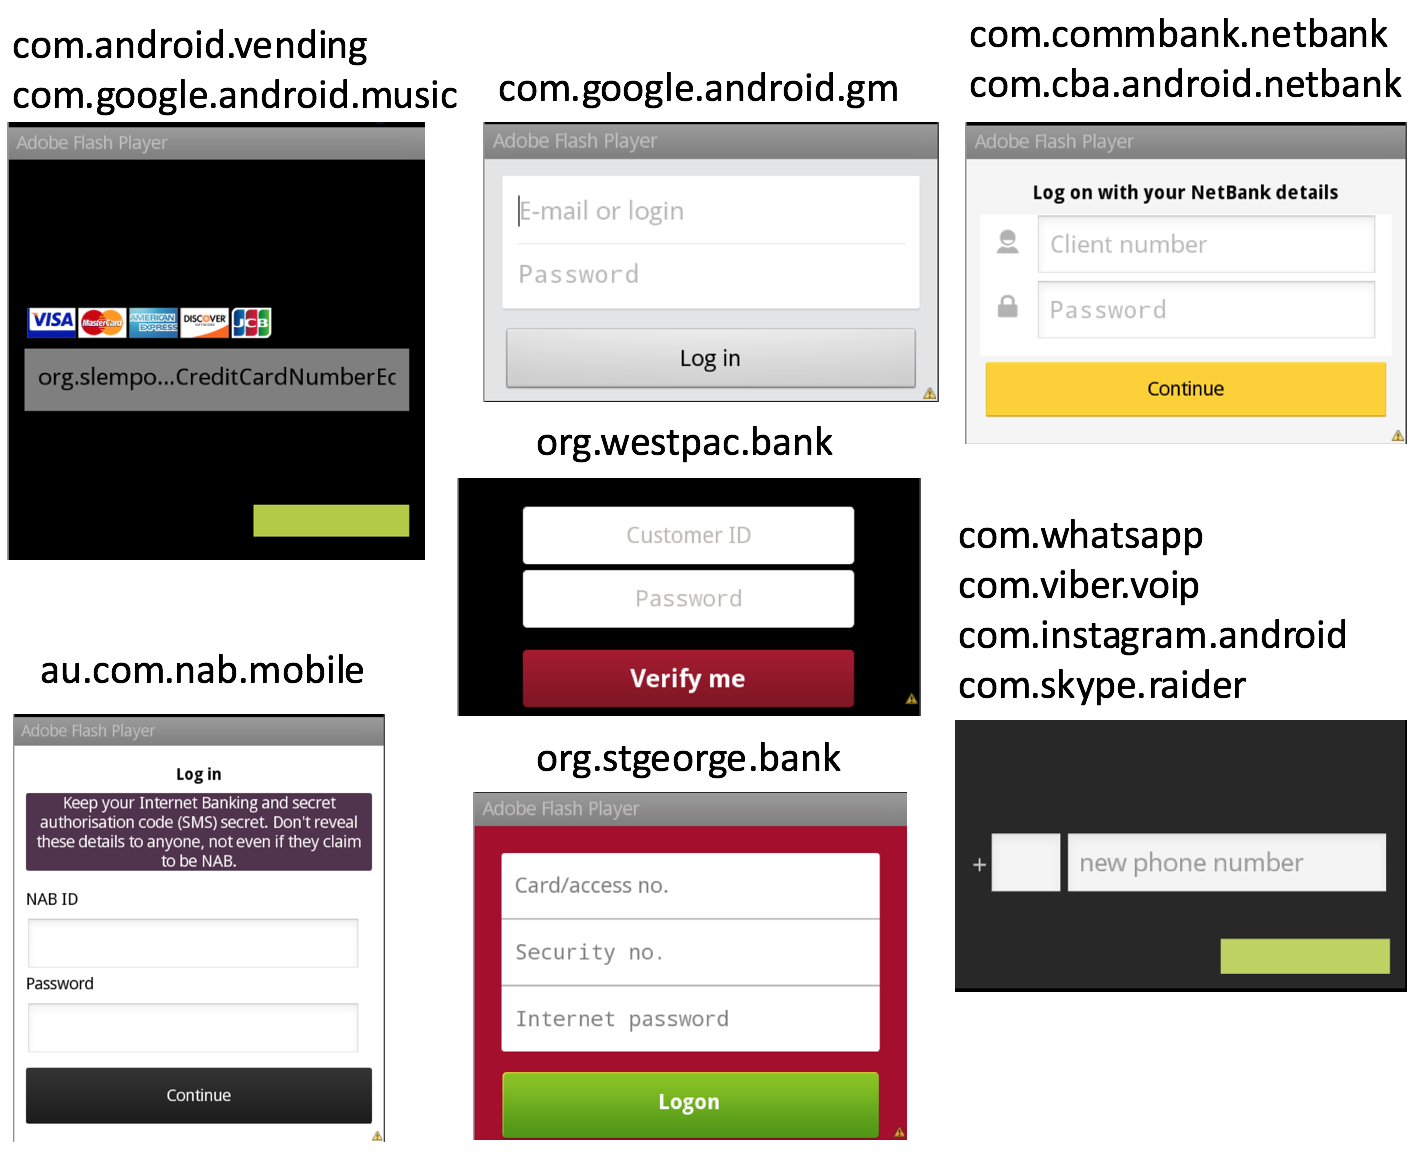
\includegraphics[width=2in]{fig/slembunkWindows.png}
  \captionof{figure}{Slembunk Phishing Windows}
  \label{fig:slembunkPhishingWindows}
\end{minipage}%
\begin{minipage}{.5\textwidth}
  \centering
  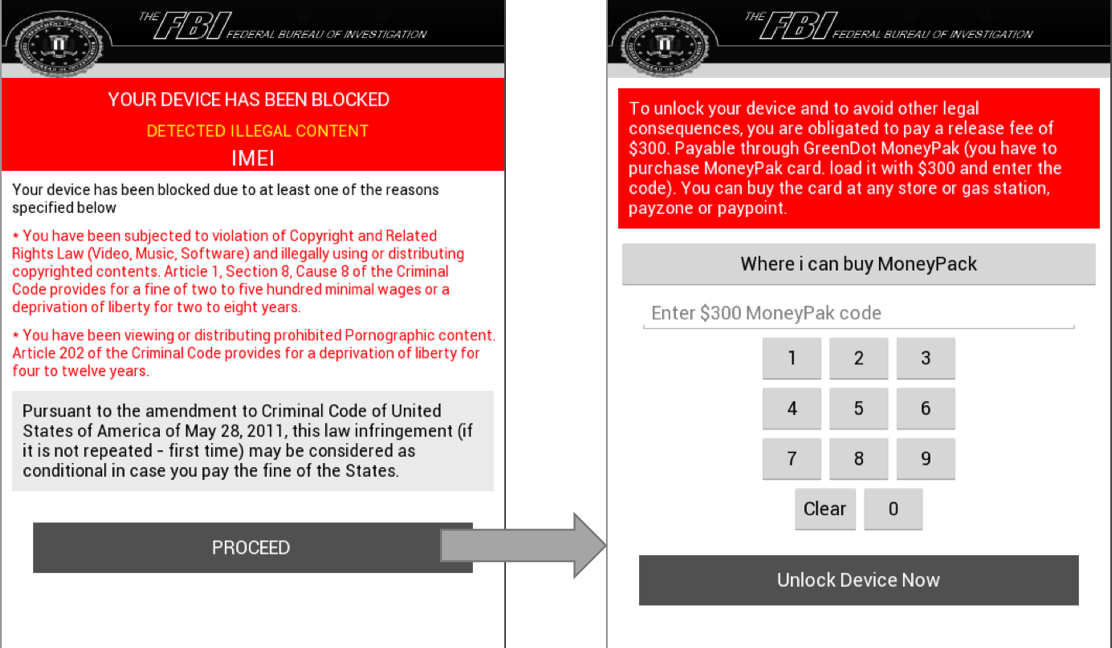
\includegraphics[width=2.35in]{fig/apleswindow.png}
  \vspace{.22in}
  \captionof{figure}{Ransom Windows by Aples}
  \label{fig:apleswindow}
\end{minipage}
\end{figure}

% Banking activities are associated with people's daily life.
Online payment and mobile wallet are becoming more popular nowadays.
Cybercriminals are also putting much effort to increase their revenue
by designing banking trojans.
%The early-stage mobile banking trojans, \eg \fn{Zitmo} work in
%combination with windows-based trojans
%to capture mTAN passwords (one-time password
%used in two-factor authentication).
In 2013, banking trojan \fn{Bankun} came into picture.
Once activated this trojan will check the 
compromised device for installed Korean banking applications,
and try to replace them with fake ones. 
%It does so by showing the victim user
%messages like ``a critical update is available for a banking app'' or
%``update is required right now.''
%The fake banking apps are well designed and look exactly the same as
%the original one. But once the user types in the banking credential,
%it will be uploaded to the cybercriminal's server.
Newer versions of banking trojans are capable of overlaying the
on-screen display of a legitimate banking app with a phishing
window.
\fn{Slembunk} falls into this category.
When this malware is activated, it will
schedule a {\em java.lang.Runnable} every 4 seconds to monitor
the current running applications by looking at the Activity
at the top of the Activity stack.
If the current running Activity belongs to certain banking
application, it will overlay a phishing window on top of the screen.
Figure~\ref{fig:slembunkPhishingWindows} shows what the phishing window
looks like for different banking applications. As an example,
if the current application is {\em com.android.vending} the left top window will be popped, and so on.
\fn{Slembunk} not only overlays phishing windows,
it is also capable of forwarding phone calls and SMS from bank
numbers, and applying the response logic.
To effectively conceal the arrival of text messages or phone calls from banks,
it will mute the device's audio system.
Later versions of \fn{Slembunk} even apply most sophisticated
string encryption and dynamic loading obfuscation techniques
(Section~\ref{sec:profile:behavior:anti}).
Recently, IBM and FireEye report~\cite{sourceCodeLeakedFireeye,sourceCodeLeakedIBM} that
the source code of \fn{SlemBunk} was leaked, which
could result in the emergence of more variants.

\vspace{-.15in}
\subsubsection{Ransom}
\label{sec:profile:monetize:ransomware}

Ransomware % is a kind of malware which is capable
locks the victim device by making it
non-responsive or encrypting its data, and
then coerces the victim to pay for the restoration.

\ptitle{Device Locking Techniques}

%\fn{FakeAV} is a fake anti-virus software.
%When it starts running, it pretends to scan victim's device.
%No matter the device is infected by malware or not,
%it will randomly choose some malware description from its database,
%and will intimidate the victim that her device is compromised,
%and to stay safe, the victim has to buy the pro version.
%If the victim keeps using the free version,
%it will use {\em AlarmManager} to periodically
%schedule a {\em BroadcastReceiver},
%which will notify the victim that the device is compromised.
%Furthermore, it will monitor victim's SMS and phone call,
%and also alerts the victim that there are viruses in the SMS or
%phone conversation is not protected.

%\begin{figure}[t]
%\centering
%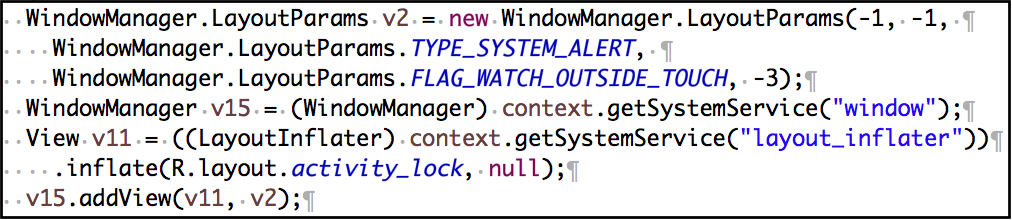
\includegraphics[width=2in]{fig/svpengInflateCodeSnippet.png}
%\vspace{-.1in}
%\caption{Svpeng Lock Screen Code Snippet}
%\label{fig:svpengInflate}
%\vspace{-.2in}
%\end{figure}

\fn{Svpeng} is both a banking trojan and ransomware.
If its C\&C server sends a command ``forceLock,''
it will lock the infected device by using SYSTEM_ALERT_WINDOW
permission and {\em WindowManager LayoutParams} 
with certain flags (\eg FLAG_SCREEN, FLAG_LAYOUT_IN_SCREEN,
FLAG_WATCH_OUTSIDE_TOUCH, \etc)
to achieve an unremovable full screen floating window.
%Figure~\ref{fig:svpengInflate} shows how it looks like
%in the code.

\fn{Aples} first appeared in 2014 -- when activated, it will
schedule a {\em Runnable} in every 0.1 second
to load the threatening window
with flag FLAG_ACTIVITY_NEW_TASK
which looks like Figure~\ref{fig:apleswindow}.
Clicking on ``PROCEED'' at the first window
will lead to the second window that asks the victim user to fill in a 
\$300 MoneyPark code to unlock.
Another malware family \fn{SimpleLocker} has applied similar techniques,
at the same time also encrypting all the data in the compromised device's external
storage using AES with a hardcoded key.

\fn{Jisut} once activated will launch a ransom window, and override {\em onKeyDown}
method of {\em Activity} to redirect key press event (\eg return key, volume key, menu key, \etc)
to some meaningless action to achieve the lock screen purpose.

\vspace{-.05in}
\ptitle{Device UnLocking Techniques}

After the victim has paid the money, the cybercriminal will tell the victim 
how to unlock the device or unlock it remotely.
The most common way is to type in the pin. 
The pin in one variety of \fn{SimpleLocker} is generated by
obtaining a serial number at beginning (which is a random number),
then uses some calculation logic (in one sample, the logic is {\em key = (serial_number - 2016)*2 + 2016}).
The second way is using remote control.
For instance, \fn{Koler} uses network command to clear a lock tag at the malware's shared preference.
The third way is by installing an unlock app.
One variety of \fn{Jisut} constantly checks whether an app with package
``{\em tk.jianmo.study}'' is installed or not; if yes, it will release the lock.

\vspace{-.2in}
\subsubsection{Aggressive Advertising}
\label{sec:profile:monetize:adware}

Mobile advertising is the main revenue source for app developers as well as
malware writers. Advertising in malware is usually more aggressive,
and this kind of apps are called adware.

\vspace{-.05in}
\ptitle{Potentially Unwanted Application (PUA)} 
A PUA adware performs tasks such as monitoring victim's personal data,
showing unwanted advertisement content,
annoying victim user with aggressive advertisement push,
showing and tempting the victim to download and install potential harmful applications.
\fn{Dowgin} is one adware app.
It will be activated once the device connectivity changes, 
user comes into presence,
or a new application is installed or deleted.
Once activated, it will display unwanted advertisements in the system's notification bar.
If the victim clicks on this notification, it will show an application wall which attracts
the victim to install new applications.
At the same time, it will send device information and the list of installed apps to a remote
C\&C server using JSON, and receive commands for showing a new advertisement,
uploading client info \etc
Many other adwares have similar behaviors, \eg \fn{Airpush}, \fn{Kuguo}, \fn{Youmi}.

\ptitle{Malware Dropper}
% A few newly found (after 2015) adware families%  try to leverage
% % root privilege and
% drop malware siliently on the infected device.
% so they are also called malware droppers.
\fn{Gorpo}, \fn{Kemoge} \cite{kemoge}, \fn{Leech} and \fn{Ztorg} are some examples.
Their task is to gain the root privilege on the infected device as discussed in 
Section~\ref{sec:profile:behavior:privilege}, and then silently drop all the active 
malware apps that are available on the ``malvertising campaign network'' to the infected device.
\fn{VikingHorde} is running in two modes: rooted and not-rooted.
If the device is not rooted, it performs in a regular fashion: uploading victim's data, 
fetch command from C\&C to execute, \etc
If the device is rooted, it will install some additional components, which are capable of 
constantly and silently downloading new malware onto the device.
We include this as part of aggressive advertising even though their main purpose
is spreading malware.

%%% Local Variables: 
%%% mode: latex
%%% TeX-master: "paper"
%%% End: 
